From a basic understanding of classical mechanics, we can determine the location of Lagrange points. But before we do any math on Lagrange points, its important to know what they are exactly. According to NASA, Lagrange points are special solutions in what is known as the ``three-body problem.'' At these points in space, the gravitational and rotational forces of the other two bodies effectively cancel each other out, allowing small objects to seemingly stay in place\autocite{JWSTOrbit}.

With this in mind, lets consider a simple system of two static masses, $m_1$ and $m_2$, where $m_1 > m_2$.

\vspace*{0.5cm}
\begin{figure}[!h]
	\centering
	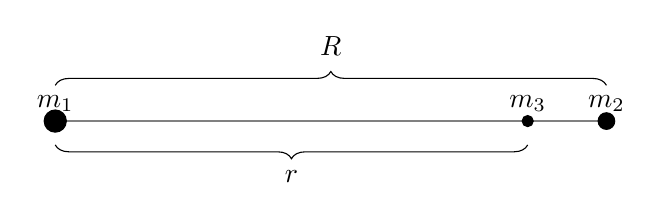
\begin{tikzpicture}
		\draw[gray,thick] (-4,0) -- (3,0);
		\filldraw (-4,0) circle (4pt) node[anchor=south]{$m_1$};
		\filldraw (3,0) circle (3pt) node[anchor=south]{$m_2$};
		\filldraw (2,0) circle (2pt) node[anchor=south]{$m_3$};
		\draw[decorate,decoration={brace,amplitude=5pt,raise=3ex}] (-4,0) -- (3,0) node[midway,yshift=27pt]{$R$};
		\draw[decorate,decoration={brace,mirror,amplitude=5pt,raise=2ex}] (-4,0) -- (2,0) node[midway,yshift=-2em]{$r$};
	\end{tikzpicture}
	\vspace*{0.25cm}
	\caption{System of two stationary bodies.}
	\label{fig:collinear-coords}
\end{figure}

In Figure \ref{fig:collinear-coords}, $R$ represents the distance between the two bodies, and $r$ represents the distance from the first body to the equilibrium point, point mass $m_3$, where the net gravitational force is 0. Using Newton's Law of Gravitation,
\begin{equation*}
	F = \frac{Gm_1m_2}{r^2}
\end{equation*}
where F is the force exerted between two bodies of mass and G is the gravitational constant, we can write the net force of the system as:
\begin{equation*}
	\frac{Gm_1m_3}{r^2} = \frac{Gm_2m_3}{(R - r)^2}
\end{equation*}
If we let $m_1 = 4m_2$ and $R = 1$, than we can directly solve for $r$:
\begin{align*}
	\frac{m_1}{r^2} &= \frac{m_2}{(R - r)^2} \\
	\left(\frac{R - r}{r}\right)^2 &= \frac{m_2}{m_1} \\
	\left(\frac{1 - r}{r}\right)^2 &= \frac{m_2}{4m_2} \\
	\frac{1 - r}{r} &= \frac{1}{2} \\
	2 - 2r &= r \\
	\frac{2}{3} &= r
\end{align*}
Of course, this scenario is not exemplary of Lagrange points, let alone the interaction between celestial bodies. Let us increase the complexity of our initial system by placing $m_2$ in a circular orbit around $m_1$. With consideration for rotational force, centripetal force is expressed as:
\begin{equation*}
	F = \frac{4\pi^2m_3r}{T^2}
\end{equation*}
where $T$ expresses the orbital period of $m_2$. Given that, from Kepler's Third Law,
\begin{equation*}
	T = 2\pi \sqrt{\frac{R^3}{G(m_1 + m_2)}}
\end{equation*}
centripetal force can be rewritten as:
\begin{equation*}
	F = \frac{G(m_1+m_2)}{R^3}m_3r \text{.}
\end{equation*}
Considering how the sign of each term of force indicates direction, the net force between $m_1$ and $m_2$ is written as:
\begin{equation*}
	F = m_3a = -\frac{Gm_1m_3}{r^2} - \frac{Gm_2m_3}{(r - R)^2} + \frac{G(m_1+m_2)}{R^3}m_3r \text{.}
\end{equation*}
By cancelling off $m_3$ to find centripetal acceleration, we get the equation:
\begin{equation*}
	a = -\frac{Gm_1}{r^2} - \frac{Gm_2}{(r - R)^2} + \frac{G(m_1+m_2)}{R^3}r \text{.}
\end{equation*}
Most of the variables are known constants, with \textit{r} being the only unknown value which represents the distance of the Lagrange point from $m_1$, given that the net radial acceleration at the point is 0.
It is worth noting that, with respect to direction, $r^2$ and $(r-R)^2$ will only reflect acceleration due to gravity in the negative direction and will not be sufficient to tell us where L1 and L3 are.
Knowing that, cautiously, $n^2 = n \times |n|$, the formula is rewritten as such to preserve the sign of $r$:
\begin{equation}
	a = -\frac{Gm_1}{r|r|} - \frac{Gm_2}{(r - R)|r - R|} + \frac{G(m_1+m_2)}{R^3}r \label{eqn:x-accel1}
\end{equation}
To save ourselves the agony of whether it is possible to algebraically solve for $r$, we will use Python to plot the centripetal acceleration with respect to distance. The Lagrange points are located where the acceleration is 0.
\begin{figure}[H]
	\centering
	\captionsetup[subfigure]{justification=centering}
	\begin{subfigure}[b]{0.4\textwidth}
		\centering
		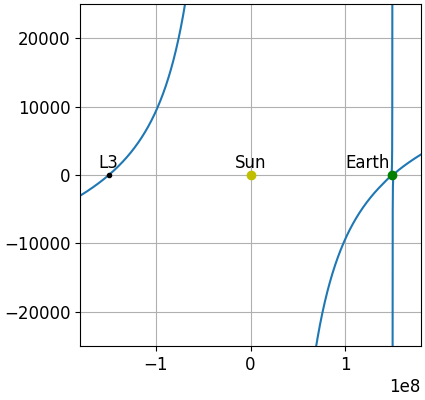
\includegraphics[scale=0.6]{figures/xyplot1.png}
		\caption{\footnotesize Radial acceleration between the Sun and Earth.}
		\label{fig:radial-accel-system}
	\end{subfigure}
	\hspace*{1cm}
	\begin{subfigure}[b]{0.4\textwidth}
		\centering
		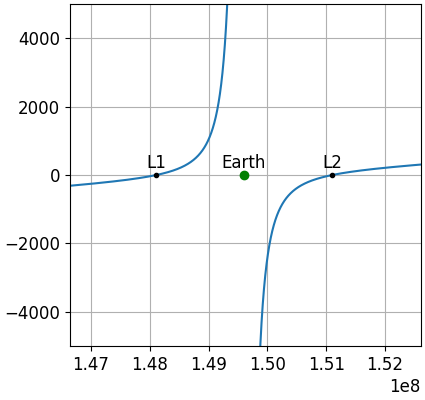
\includegraphics[scale=0.6]{figures/xyplot2.png}
		\caption{\footnotesize Radial acceleration around the Earth.\vspace*{1.16em}}
		\label{fig:radial-accel-earth}
	\end{subfigure}
	\label{fig:radial-accel}
	\caption{Net radial acceleration vs distance of the Sun-Earth system. Graphs are created using the Matplotlib Python library.}
\end{figure}
Given that we are only concerned with L2, the distance of L2 from the Sun is computed as $1.511 \times 10^8 \si{\kilo\metre}$.

Note how Equation \eqref{eqn:x-accel1} for acceleration is dependent on the distance an object is from either body.
Should we try to predict the motion of an object, there would be no way to express distance as a function of time as it is dependant on acceleration.
This is a major hurdle that occurs in physics and, while there can be specific situations where this can be overcome, most of the time there is no solution.
We should not let this caveat daunt us, however, as there is still a lot to learn about how we describe the motion of objects in such a relation.

\newpage
